\documentclass[xcolor=table]{beamer}

% -----------General Settings ------------
\usetheme{default}
\usetheme{Antibes}
\usecolortheme{dolphin}
\setbeamercolor{normal text}{bg=blue!3}
\beamertemplatetransparentcovereddynamicmedium
\beamertemplateshadingbackground{blue!4}{black!8}
\graphicspath{{./images/}} %images path
\title[Image Processing to Detect Worms]{Image Processing to Detect Worms}
\author[Javier Fern\'andez]{Javier Fern\'andez}
\institute[Uppsala University]{Uppsala University. Uppsala, Sweden}

\begin{document}
\maketitle

%----------- Introduction ----------------

\section{Introduction}
\subsection{C.elegans}

\begin{frame}{Caenorhabditis elegans (C.elegans)}

\begin{itemize}
  \item itemized item 1 \pause 
  \item itemized item 2 \pause
  \item itemized item 3
\end{itemize}

\end{frame}

\subsection{Motivation}
\begin{frame}{The problem: Motivation}

\begin{itemize}
  \item itemized item 1 
  \item itemized item 2 
  \item itemized item 3
\end{itemize}

\end{frame}
\subsection{Purpose}
\begin{frame}{The problem: Purpose}

\begin{itemize}
  \item itemized item 1 
  \item itemized item 2 
  \item itemized item 3
\end{itemize}

\end{frame}

\subsection{Background}
\begin{frame}{Background on Worm Detection}

\begin{itemize}
  \item itemized item 1 
  \item itemized item 2 
  \item itemized item 3
\end{itemize}

\end{frame}

% -----------------------------------------

\subsection{Objectives}
\begin{frame}{Objectives}

\large \textbf{General Objective}\\
\vskip7pt

\begin{itemize}
  \item itemized item 1 \pause 
\end{itemize}

\vskip7pt
\pause \large \textbf{Specific Objectives}\\
\vskip7pt

\begin{itemize}
  \item itemized item 1 \pause 
  \item itemized item 2 \pause
  \item itemized item 3
\end{itemize}

\end{frame}

%-----------------------------------------

\section{Methodology}
\subsection{Solution Methodology Flowchart}
\begin{frame}{}

\begin{figure}[h t b p ! H]
 \centering
   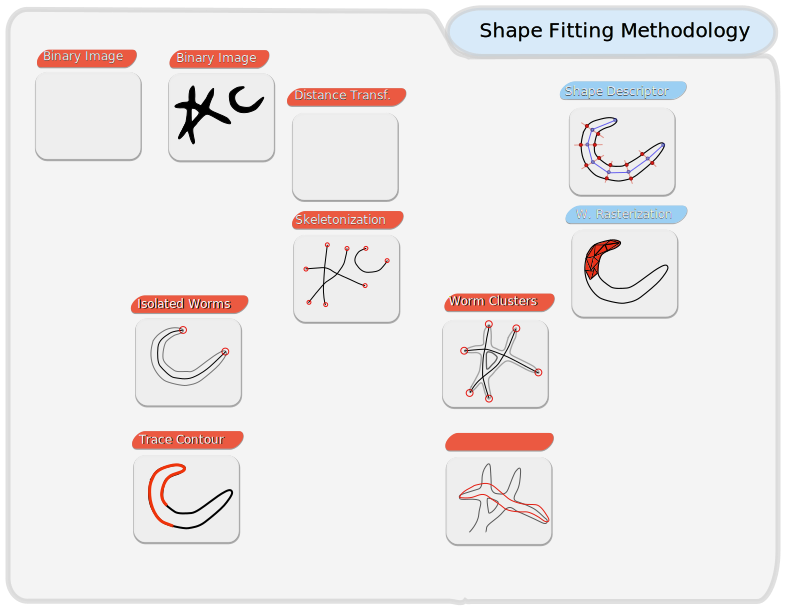
\includegraphics[scale=0.46]{diagrams/design.pdf}
\end{figure}
\end{frame}


% -------- Original and Thresholding -----------

\subsection{Thresholding}
\begin{frame}{Thresholding}

\begin{columns}[c]
\column{1.5in}
\includegraphics[scale=0.27]{original}
\column{1.5in}
\includegraphics[scale=0.27]{thres/worms}

\end{columns}

\end{frame}

% -------- Distance Transformation  -----------

\subsection{Distance Transformation}
\begin{frame}{Distance Transformation: Manhattan Distance}

\begin{columns}[c]
\column{2.4in}
\begin{itemize}
\item Improve skeletonization algorithm \pause
\item Trace contour of isolated worms \pause
\item Automatic calculation of worm profile \pause
\item Path guessing algorithm
\end{itemize}
\column{2in}
\includegraphics[scale=0.27]{results/test1/dt-shape1}

\end{columns}

\end{frame}


% -------- Skeletonization  -----------

\subsection{Skeletonization}
\begin{frame}{Worm Skeletonization}

\begin{columns}[c]
\column{2.4in}
\begin{itemize}
\item Thinning Algorithm $+$ Distance Map \pause
\item 1 pixel thick paths that tend to the medial axes \pause
\item Skeleton endpoint expansion and Worm Endpoint detection \pause
\item Segmentation in groups
\end{itemize}
\column{2in}
\includegraphics[scale=0.3]{skeleton1}

\end{columns}

\end{frame}


% -------- Shape Matching  -----------

\subsection{Shape Matching}
\begin{frame}{Isolated Worms}

\begin{columns}[c]
\column{2.4in}
\begin{itemize}
\item Contour can be traced easily.The shape is rasterized 
and thus fitted \pause
\item Worm Profiling 
\end{itemize}
\column{2.2in}
\includegraphics[scale=0.5]{iso}
\end{columns}

\end{frame}

% -------- Shape Matching  -----------

\subsection{Shape Matching}
\begin{frame}{Worm Cluster: Matching Approach}

\begin{columns}[c]
\column{2.6in}
\begin{itemize}
\item Calculate feasible worm paths from every endpoint
  \begin{itemize}
  \item Paths no longer than 1.5 of the average worm size
  \item Path guessing algorithm 
  \end{itemize}
\pause\item A worm shape is constructed given a path and a worm
  profile \pause
\item The shape is deformed until the best possible match is
  found \pause
\item For this is required: a shape descriptor, a
  rasterization method, distance measure between shapes
  and a optimization approach.
\end{itemize}
\column{2.2in}
\includegraphics[scale=0.3]{clusterskeleton}
\end{columns}

\end{frame}


% -------- Shape Matching  -----------

\subsection{Shape Matching}
\begin{frame}{Worm Shape Descriptor}

\begin{columns}[c]
\column{2.0in}
\begin{itemize}
\item Set of control points connected by straight lines \pause
\item Bisectors of control point angles \pause
\item Calculate contour points from the worm profile \pause
\item Trace the contour through a Cardinal Spline \\
\item The shape is rasterized by triangulating the area and 
  rasterizing each triangle individually.
\end{itemize}
\column{2.3in}
\includegraphics<1>[scale=0.45]{control}
\includegraphics<2>[scale=0.45]{bisec}
\includegraphics<3>[scale=0.45]{prof}
\includegraphics<4->[scale=0.45]{shape}
\end{columns}

\end{frame}

% -------- Shape Matching  -----------

\subsection{Shape Matching}
\begin{frame}{Matching Optimization}

  \begin{itemize}
  \item A worm shape is generated given a skeleton path \pause
  \item The shape is deformed until the distance between the shape and the image 
    is minimized, thus obtaining a worm conformation. \pause
  \item The distance is measured through an Energy Formulation defined as the
    sum of the External and Internal energy. \pause
    \begin{itemize}
    \item External: How well the model matches the data \pause
    \item Internal: Model resistance to be pushed into not coherent directions
    \end{itemize}\pause
  \item The best set of conformations is chosen: maximizing the amount of covered
    endpoints and minimizing the total energy \pause
  \item Incorrect conformations can be easily fixed manually
  \end{itemize}

\end{frame}

%---------------- Results ---------------

\section{Results}
\subsection{Test Set}
\begin{frame}{Test Set: test Image 1}

  \begin{itemize}
  \item Images in increasing difficulty level: number of worms
    and overlaps
  \end{itemize}

\begin{table}[h]
\begin{center}
\begin{tabular}[h]{|c|c|c|c|c|}
    \hline
    \rowcolor{gray!35}
    Test & Isolated & Clusters & Clustered Worms & Total\\
    Test 1 & 11/19 (57.8\%) & 3 & 8/19 (42.1\%) & 19 \\
    \hline
  \end{tabular}
\end{center}
\end{table}

\begin{center}
\includegraphics[scale=0.25]{results/test1/original}
\end{center}

\end{frame}

\begin{frame}{Test Set: test Image 2}

  \begin{itemize}
  \item Images in increasing difficulty level: number of worms
    and overlaps
  \end{itemize}

\begin{table}[h]
\begin{center}
\begin{tabular}[h]{|c|c|c|c|c|}
    \hline
    \rowcolor{gray!35}
    Test & Isolated & Clusters & Clustered Worms & Total\\
    Test 2 & 8/33 (24.2\%) & 3 & 25/33 (75.7\%)& 33 \\    
    \hline
  \end{tabular}
\end{center}
\end{table}


\begin{center}
\includegraphics[scale=0.22]{results/test2/original2}
\end{center}

\end{frame}

\begin{frame}{Test Set: test Image 3}

  \begin{itemize}
  \item Images in increasing difficulty level: number of worms
    and overlaps
  \end{itemize}

\begin{table}[h]
\begin{center}
\begin{tabular}[h]{|c|c|c|c|c|}
    \hline
    \rowcolor{gray!35}
    Test & Isolated & Clusters & Clustered Worms & Total\\
    Test 3 & 13/38 (34.2\%)& 5 & 25/38 (65.7\%) & 38 \\
    \hline
  \end{tabular}
\end{center}
\end{table}

\begin{center}
\includegraphics[scale=0.25]{results/test3/original3}
\end{center}
\end{frame}

% ------ Matching Results ------

\subsection{Matching Results}
\begin{frame}{Matching Experiments}

  \begin{itemize}
  \item Automated matching. 
    \begin{itemize}
    \item Two different path sets: With and without Path Guessing 
    \item Missing endpoints 
    \end{itemize}
  \end{itemize}

\end{frame}

\begin{frame}{Matching Results: Test Image 1}

\begin{scriptsize}
\begin{table}[h]
\begin{center}
\begin{tabular}[h]{|c|c|c|c|c|}
    \hline
    \rowcolor{gray!35}
    Path finding & Iso. Matching & Cluster Matching 
    & Total
    & Time (s) \\ 
    \hline  
    Every Path - me & 8/8 (100\%) & 7/25 (28\%) & 15/33 (45.4\%) & 21.8 \\ 
    \hline
    P.Guessing - me & 8/8 (100\%) & 10/25 (40\%) & 18/33 (54.5\%) & 23.7\\
    \hline
    Every Path + me & 8/8 (100\%)& 15/23 (65.2\%) & 23/33 (69.7\%)& 42.3 \\
    \hline
    P.Guessing + me & 8/8 (100\%)& 21/25 (84\%) & 29/33 \alert{(87.8\%)} & 45 \\
    \hline
  \end{tabular}
\end{center}
\end{table}
\end{scriptsize}

\end{frame}


\end{document}